\documentclass{beamer}
\usepackage[T2A]{fontenc}
\usepackage[utf8]{inputenc}
\usepackage[russian]{babel}
\usepackage{graphicx}
\usepackage{hyperref}
\usetheme{default}
\usecolortheme{dove}

\title{Стандарты сжатия видео H.264, MPEG-4 AVC}
\author{Степан Долгоруков, КБ-501 \\ \small \texttt{Stepan.Dolgorukov@urfu.me}}
\institute{УрФУ ИЕНиМ ДММиКН}
\date{12 мая 2026 г.}

\begin{document}
	\setbeamertemplate{caption}[numbered]
	
	\begin{frame}
		\titlepage
	\end{frame}

	\begin{frame}{Основные определения}
		\textbf{Пиксель} (\textbf{pic}ture \textbf{el}ement) --- неделимый элемент изображения.
		\textbf{Изображение} --- матрица пикселей.
		
		\textbf{Видео} --- кортёж (конечная последовательность) изображений.

		\textbf{Кадр} --- член (элемент, компонента) кортежа изображений, являющегося видео.
		
		\textbf{Битрейт} --- количество информации одного кадра, демонстрируемого за единицу времени. Чаще всего, единица измерения битрейта --- бит в секунду (бит/с).
	\end{frame}
	
	\begin{frame}{Проблема}
		\begin{itemize}
			\item \textbf{Языком практическим}: нахождение наилучшего (оптимального) метода кодирования видео с учётом ограничений носителей информации (информационный объём, пропускная способность).
			
			\item \textbf{Языком теоретическим}: уменьшение количества информации, требующегося для однозначного представлени кортежа матриц пикселей.
		\end{itemize}
	\end{frame}
	
	\begin{frame}{Избыточность информации}
		\begin{itemize}
			\item \textbf{Пространственная} --- дублирование информации в кадре.
		
			\item \textbf{Временная} --- дублирование информации в видео.
		\end{itemize}
		
		\begin{figure}
			\centering
			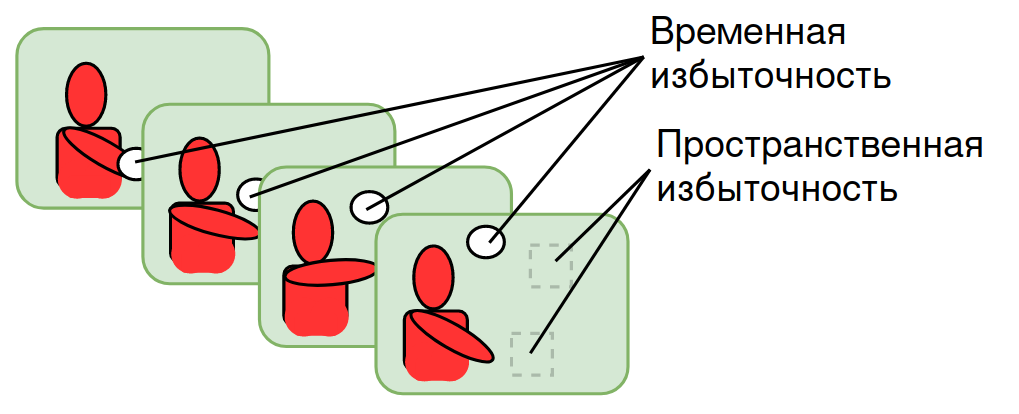
\includegraphics[width=0.7\linewidth]{image.EYP3O3}
			\caption{Пример наличия временных, пространственных избыточностей в видео, состоящего из 4-ёх кадров}
		\end{figure}
	\end{frame}
	
	\begin{frame}{Типы сжатия}
		\begin{itemize}
			\item \textbf{$\delta$-сжатие (межкадровое)} --- хранение или передача разницы (diff) между кадрами. Операция вычисления разницы не является коммутативной. Поэтому необходимо определить, какой кадр является from-кадром, а какой to-кадром. Чем более похожи кадры, тем меньшего количества информации занимают различия.
		
			\item \textbf{Пространственное (внутрикадровое)} ---
			\begin{itemize}
				\item разбиение на блоки;
				\item предсказание пикселя по соседним пикселям;
				\item исключение незначительных деталей;
				\item энтропийное кодирование (применение кодов переменной длины).
			\end{itemize}
		\end{itemize}
	\end{frame}
	
	\begin{frame}{Стандарт H.264}
		H.264, MPEG-4 Part 10 (ISO/IEC 14496-10) --- \textbf{технически идентичные стандарты}. Текст технической спецификации общедоступен.
		
		H.264 --- имя в соответствии с соглашениями об именах в ITU (International Telecommunication Union), MPEG 4 Part 10 --- имя в соответствии с соглашениями об именах в ISO (International Organization for Standartization)/IEC (International Electronechnical Commission).
		
		\textbf{Коммерческое применение требует выплаты роялти} (платежи за право применение интеллектуальной собственности). \textbf{Применение H.264 не требует выплаты роялти, если видео предоставляется потребителю бесплатно}.
	\end{frame}
	
	\begin{frame}{Макроблок}
		Для уменьшения времени вычисления кода, задающего видео, кодировщик может обрабатывать кадр блоками пикселей. Макроблок --- квадратный фрагмент кадра.
	\end{frame}
	
	\begin{frame}{Адаптивное разбиение кадра в H.264}
		Кодировщик, действующий в соответствии с H.264, анализирует участок изображения для выбора оптимального размера макроблока для этого участка.
		
		Наибольший размер макроблока в H.264 --- $16\times16$ пикселей, наменьший --- $4\times4$.
		
		\begin{figure}
			\centering
			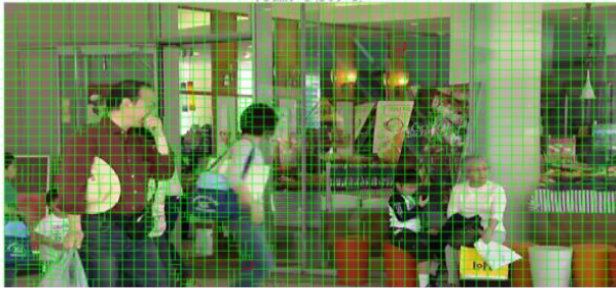
\includegraphics[width=0.7\linewidth]{image.0EGIP3}
			\caption{Кадр, являющийся пример того, что размер макроблока в H.264 --- динамическая величина}
		\end{figure}
	\end{frame}
	
	\begin{frame}{Тип кадра в H.264}
		\begin{itemize}
			\item \textbf{Тип I (Интра-кодированные)} --- кодируются независимо от других кадров.
			\item \textbf{Тип P (Прогнозируемо-кодированные)} --- кодируются с ссылками на макроблоки в предшествующих кадрах. Ссылка может быть как на макроблок из кадра типа I, так и на макроблок из кадра типа P.
			\item \textbf{Тип B (Би-направленно-прогнозируемо-кодированные)} --- кодируются с ссылками на предшествующие, на последующие кадры.
		\end{itemize}
		
		\begin{figure}
			\centering
			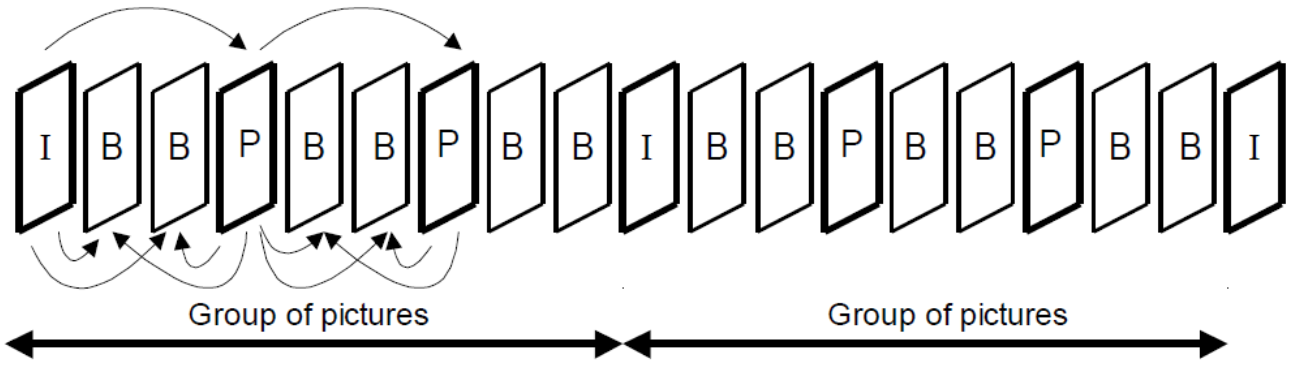
\includegraphics[width=0.7\linewidth]{image.DURGP3}
			\caption{Примеры присвоения типов кадрам (расставлены не все ссылки)}
		\end{figure}
	\end{frame}
	
	\begin{frame}{Энтропийное кодирование в H.264}
		Выбор из 2-ух алгоритмов:
		\begin{itemize}
			\item \textbf{CABAC} (Контекстно-адаптивное двоичное арифметическое кодирование) --- арифметическое кодирование: представление всей информации в виде дробного числа.
			\item \textbf{CAVLC} (Контекстно-адаптивное кодирование с кодами переменной длины) --- кодирование, основывающееся на кодах Хаффмана.
		\end{itemize}
	\end{frame}
	
	\begin{frame}{Сжатие в H.264}
		\begin{enumerate}
			\item Устранение избыточностей внутри кадра, между кадрами;
			\item Перевод информации из пикселей в набор частот;
			\item Исключение незначительных частот;
			\item Энтропийное кодирование.
		\end{enumerate}
	\end{frame}
	
	\begin{frame}{Проведение вычислительного эксперимента}
		Значения показательных характеристик исходного файла, содержащего видео:
		\begin{itemize}
			\item Кодек видео: HEVC (H.265);
			\item Количество кадров в видео: 439;
			\item Битрейт: 20213223 бит/с;
			\item Информационный объём файла: 37011418 байтов.
		\end{itemize}
		
		Значения показательных характеристик машины, на которой производилось кодирование:
		\begin{itemize}
			\item CPU: Intel Core Ultra 7 155H;
			\item Информационный объём ОЗУ: 15825216 байтов;
			\item ОС: Pop! OS 22.04 LTS.
		\end{itemize}
	\end{frame}
		
	\begin{frame}{Проведение вычислительного эксперимента}
		\begin{table}[h]
			\centering
			\small
			\begin{tabular}{|c|c|c|c|}
				\hline
				Кодек 		 	& Реализация	& Время кодир-я, сек.	& Размер файла, Б \\ \hline
				H.264			& libx264		& 51.55				  	& 37098002 \\ \hline
				MPEG-2 Video 	& mpeg2video	& 13.54               	& 37476352 \\ \hline
				MPEG-4 Part2    & mpeg4    		& 9.90					& 37400878 \\ \hline
				AV1				& libaom1		& 14334.48				& 13728613	\\ \hline
				VP8				& libvpx		& 78.65					& 19602287 \\ \hline
				VP9				& libvpx-vp9	& 277.37				& 26440826 \\ \hline
				MJPEG			& mjpeg			& 16.13					& 36295936 \\ \hline
				ProRes			& prores\_ks	& 109.79				& 1687378350 \\ \hline
				FFV1			& ffv1			& 23.74					& 404208749 \\ \hline
			\end{tabular}
			\caption{Таблица результатов кодирования}
		\end{table}
		
		Исходный текст этой презентации, программы командной оболочки Bash для проведения эксперимента, инструкция для запуска программ опубликованы в репозитории на GitHub: \url{https://github.com/stepan-dolgorukov/h264-rept}.
	\end{frame}
\end{document}
